\documentclass[14 pt,xcolor=dvipsnames]{beamer}

\usepackage{epsdice}

\usepackage[absolute,overlay]{textpos}

\usepackage[orientation=portrait,size=custom,width=25.4,height=19.05]{beamerposter}

%25,4 см 19,05 см размеры слайда в powerpoint

\usetheme{metropolis}
\metroset{
  %progressbar=none,
  numbering=none,
  subsectionpage=progressbar,
  block=fill
}

%\usecolortheme{seahorse}

\usepackage{fontspec}
\usepackage{polyglossia}
\setmainlanguage{russian}


\usepackage{fontawesome5} % removed [fixed]
\setmainfont[Ligatures=TeX]{Myriad Pro}
\setsansfont{Myriad Pro}


\usepackage{amssymb,amsmath,amsxtra,amsthm}


\usepackage{unicode-math}
\usepackage{centernot}

\usepackage{graphicx}
\graphicspath{{img/}}

\usepackage{wrapfig}
\usepackage{animate}
\usepackage{tikz}
%\usetikzlibrary{shapes.geometric,patterns,positioning,matrix,calc,arrows,shapes,fit,decorations,decorations.pathmorphing}
\usepackage{pifont}
\usepackage{comment}
\usepackage[font=small,labelfont=bf]{caption}
\captionsetup[figure]{labelformat=empty}
\includecomment{techno}

\usefonttheme[onlymath]{serif}


%Расположение

\setbeamersize{text margin left=15 mm,text margin right=5mm} 
\setlength{\leftmargini}{38 pt}

%\usepackage{showframe}
%\usepackage{enumitem}
%\setlist{leftmargin=5.5mm}


%Цвета от дирекции

\definecolor{dirblack}{RGB}{58, 58, 58}
\definecolor{dirwhite}{RGB}{245, 245, 245}
\definecolor{dirred}{RGB}{149, 55, 53}
\definecolor{dirblue}{RGB}{0, 90, 171}
\definecolor{dirorange}{RGB}{235, 143, 76}
\definecolor{dirlightblue}{RGB}{75, 172, 198}
\definecolor{dirgreen}{RGB}{155, 187, 89}
\definecolor{dircomment}{RGB}{128, 100, 162}

\setbeamercolor{title separator}{bg=dirlightblue!50, fg=dirblue}

%Цвета блоков

\setbeamercolor{block title}{bg=dirblue!30,fg=dirblack}

\setbeamercolor{block title example}{bg=dirlightblue!50,fg=dirblack}

\setbeamercolor{block body example}{bg=dirlightblue!20,fg=dirblack}

\AtBeginEnvironment{exampleblock}{\setbeamercolor{itemize item}{fg=dirblack}}
%\setbeamertemplate{blocks}[rounded][shadow]

% Набор команд для удобства верстки

\newcommand{\RR}{\mathbb{R}}
\newcommand{\ZZ}{\mathbb{Z}}
\newcommand{\la}{\lambda}

% Набор команд для структуризации

%\newcommand{\quest}{\faQuestionCircleO}
%\faPencilSquareO \faPuzzlePiece \faQuestionCircleO  \faIcon*[regular]{file} {\textcolor{dirblue}
%\newcommand{\quest}{\textcolor{dirblue}{\boxed{\textbf{?}}}
\newcommand{\task}{\faIcon{tasks}}
\newcommand{\exmpl}{\faPuzzlePiece}
\newcommand{\dfn}{\faIcon{pen-square}}
\newcommand{\quest}{\textcolor{dirblue}{\faQuestionCircle[regular]}}
\newcommand{\acc}[1]{\textcolor{dirred}{#1}}
\newcommand{\accm}[1]{\textcolor{dirred}{#1}}
\newcommand{\acct}[1]{\textcolor{dirblue}{#1}}
\newcommand{\acctm}[1]{\textcolor{dirblue}{#1}}
\newcommand{\accex}[1]{\textcolor{dirblack}{\bf #1}}
\newcommand{\accexm}[1]{\textcolor{dirblack}{ \mathbf{#1}}}
\newcommand{\acclp}[1]{\textcolor{dirorange}{\it #1}}


\newcommand{\videotitle}[1]{\begin{center}
    \textcolor{dirblue}{#1}

    \todo{название видеофрагмента}
\end{center}}

\newcommand{\lecturetitle}[1]{\begin{center}
    \textcolor{dirblue}{#1}

    \todo{название лекции}
\end{center}}




\newcommand{\todo}[1]{\textcolor{dircomment}{\bf #1}}

\newcommand{\spcbig}{\vspace{-10 pt}}
\newcommand{\spcsmall}{\vspace{-5 pt}}

%\usepackage{listings}
%\lstset{
%xleftmargin=0 pt,
%  basicstyle=\small, 
%  language=Python,
  %tabsize = 2,
%  backgroundcolor=\color{mc!20!white}
%}



%\newcommand{\mypart}[1]{\begin{frame}[standout]{\huge #1}\end{frame}}

\setbeamercolor{background canvas}{bg=}

% frame title setup
\setbeamercolor{frametitle}{bg=,fg=dirblue}
\setbeamertemplate{frametitle}[default][left]

\addtobeamertemplate{frametitle}{\hspace*{-0.5 cm}}{\vspace*{0.25cm}}


%Шрифты
\setbeamerfont{frametitle}{family=\rmfamily,series=\bfseries,size={\fontsize{33}{30}}}
\setbeamerfont{framesubtitle}{family=\rmfamily,series=\bfseries,size={\fontsize{26}{20}}}





\usepackage{physics}
\newcommand{\R}{\mathbb{R}}

\usepackage[outline]{contour}


\usepackage{pgfplots}
\pgfplotsset{colormap/viridis}


\pgfplotsset{compat=newest}

\usepackage{tikz}
\usetikzlibrary{calc}
\usetikzlibrary{quotes,angles}
\usetikzlibrary{arrows}
\usetikzlibrary{arrows.meta}
\usetikzlibrary{positioning,intersections,decorations.markings}
\usetikzlibrary{patterns}

\usepackage{tkz-euclide} 

\newcommand{\grid}{\draw[color=gray,step=1.0,dotted] (-2.1,-2.1) grid (9.6,6.1)}

\newcommand{\ba}{\symbf{a}}
\newcommand{\be}{\symbf{e}}
\newcommand{\bb}{\symbf{b}}
\newcommand{\bc}{\symbf{c}}
\newcommand{\bd}{\symbf{d}}
\newcommand{\bx}{\symbf{x}}
\newcommand{\bv}{\symbf{v}}
\newcommand{\Lin}{\mathrm{Lin}}

\DeclareMathOperator{\Span}{Span}
\DeclareMathOperator{\LL}{L}

%\tikzset{>=latex}

\colorlet{veca}{red}
\colorlet{vecb}{blue}
\colorlet{vecc}{olive}


\tikzset{cross/.style={cross out, draw=black, minimum size=2*(#1-\pgflinewidth), inner sep=0pt, outer sep=0pt},
	%default radius will be 1pt. 
	cross/.default={10pt}}


\begin{document}


\begin{frame} % название лекции

\lecturetitle{Шаблон для тестов и экспериментов}

\end{frame}




\begin{frame}{RX1}
	
	
	\begin{figure}[H]
		\noindent\makebox[\textwidth][c]{%
			\begin{minipage}[H]{0.5\linewidth}
				\begin{figure}
				\centering
					\caption{Джин Говард Голуб}
					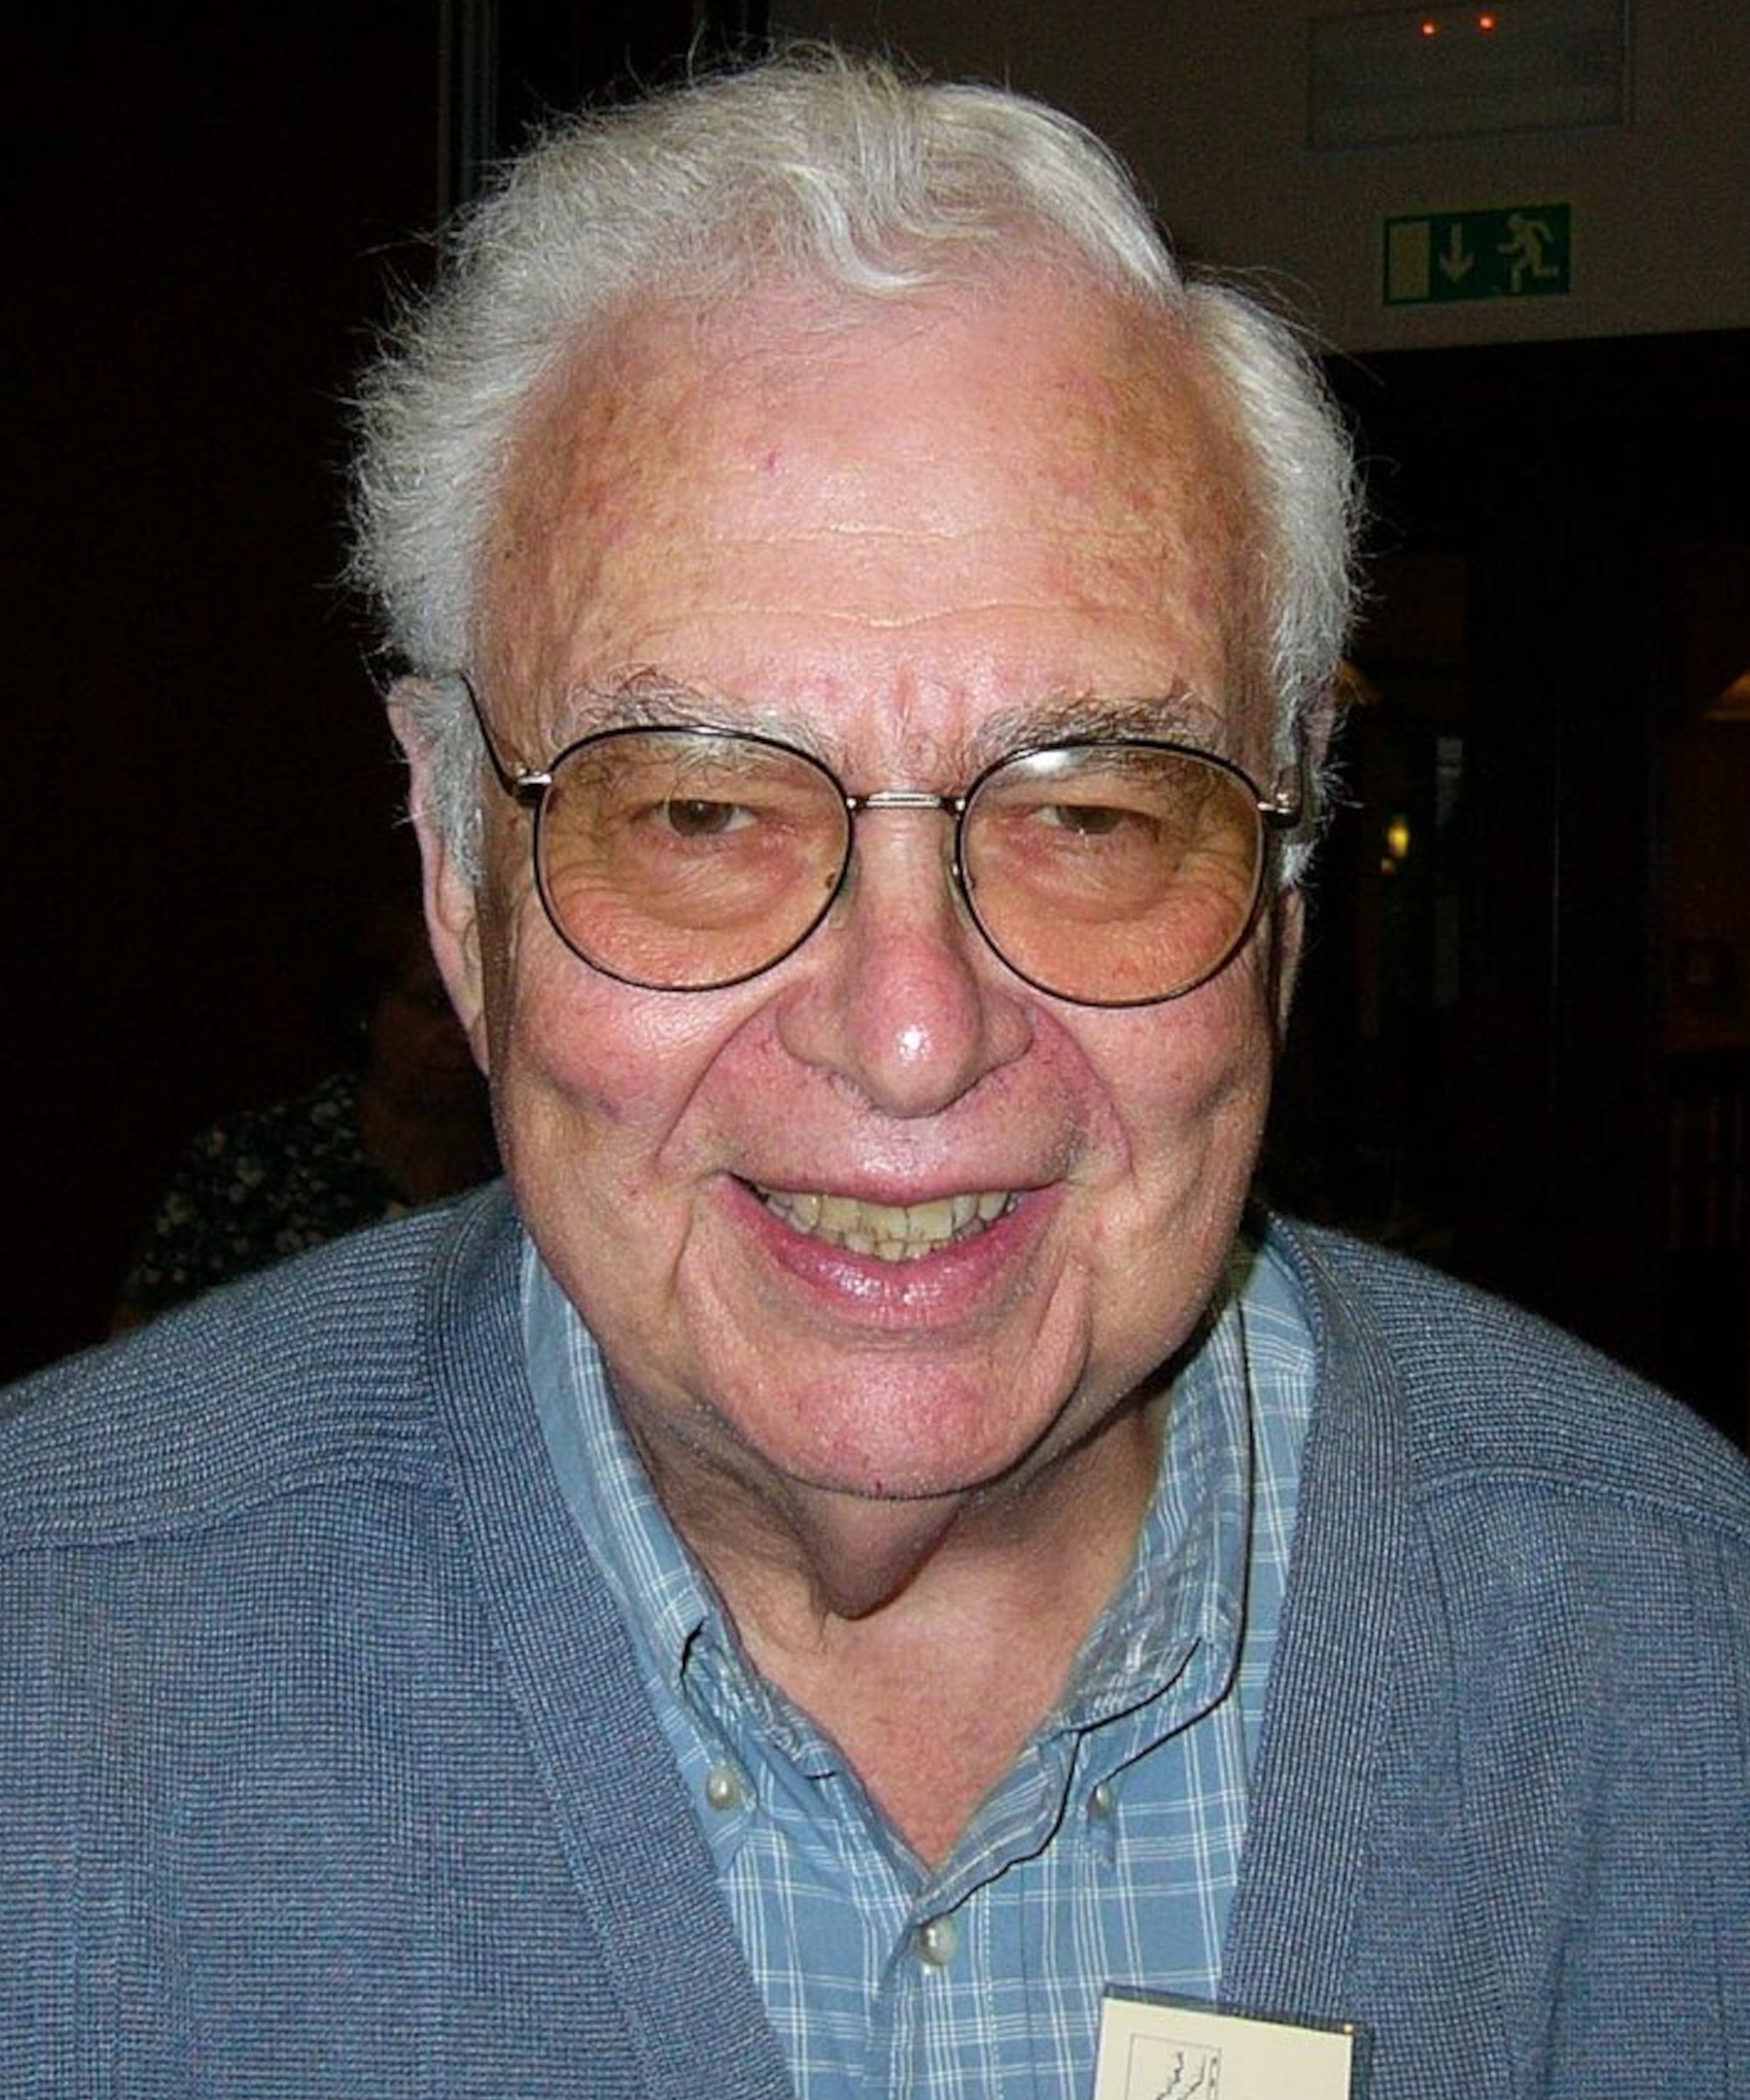
\includegraphics[width=0.7\linewidth]{pic_genegolub}
					\label{fig:picgenegolub}
				\end{figure}
			\end{minipage}
			\begin{minipage}[H]{0.5\linewidth}
				\begin{figure}
					\centering
					\caption{Уильям Мортон Кэхэн}
					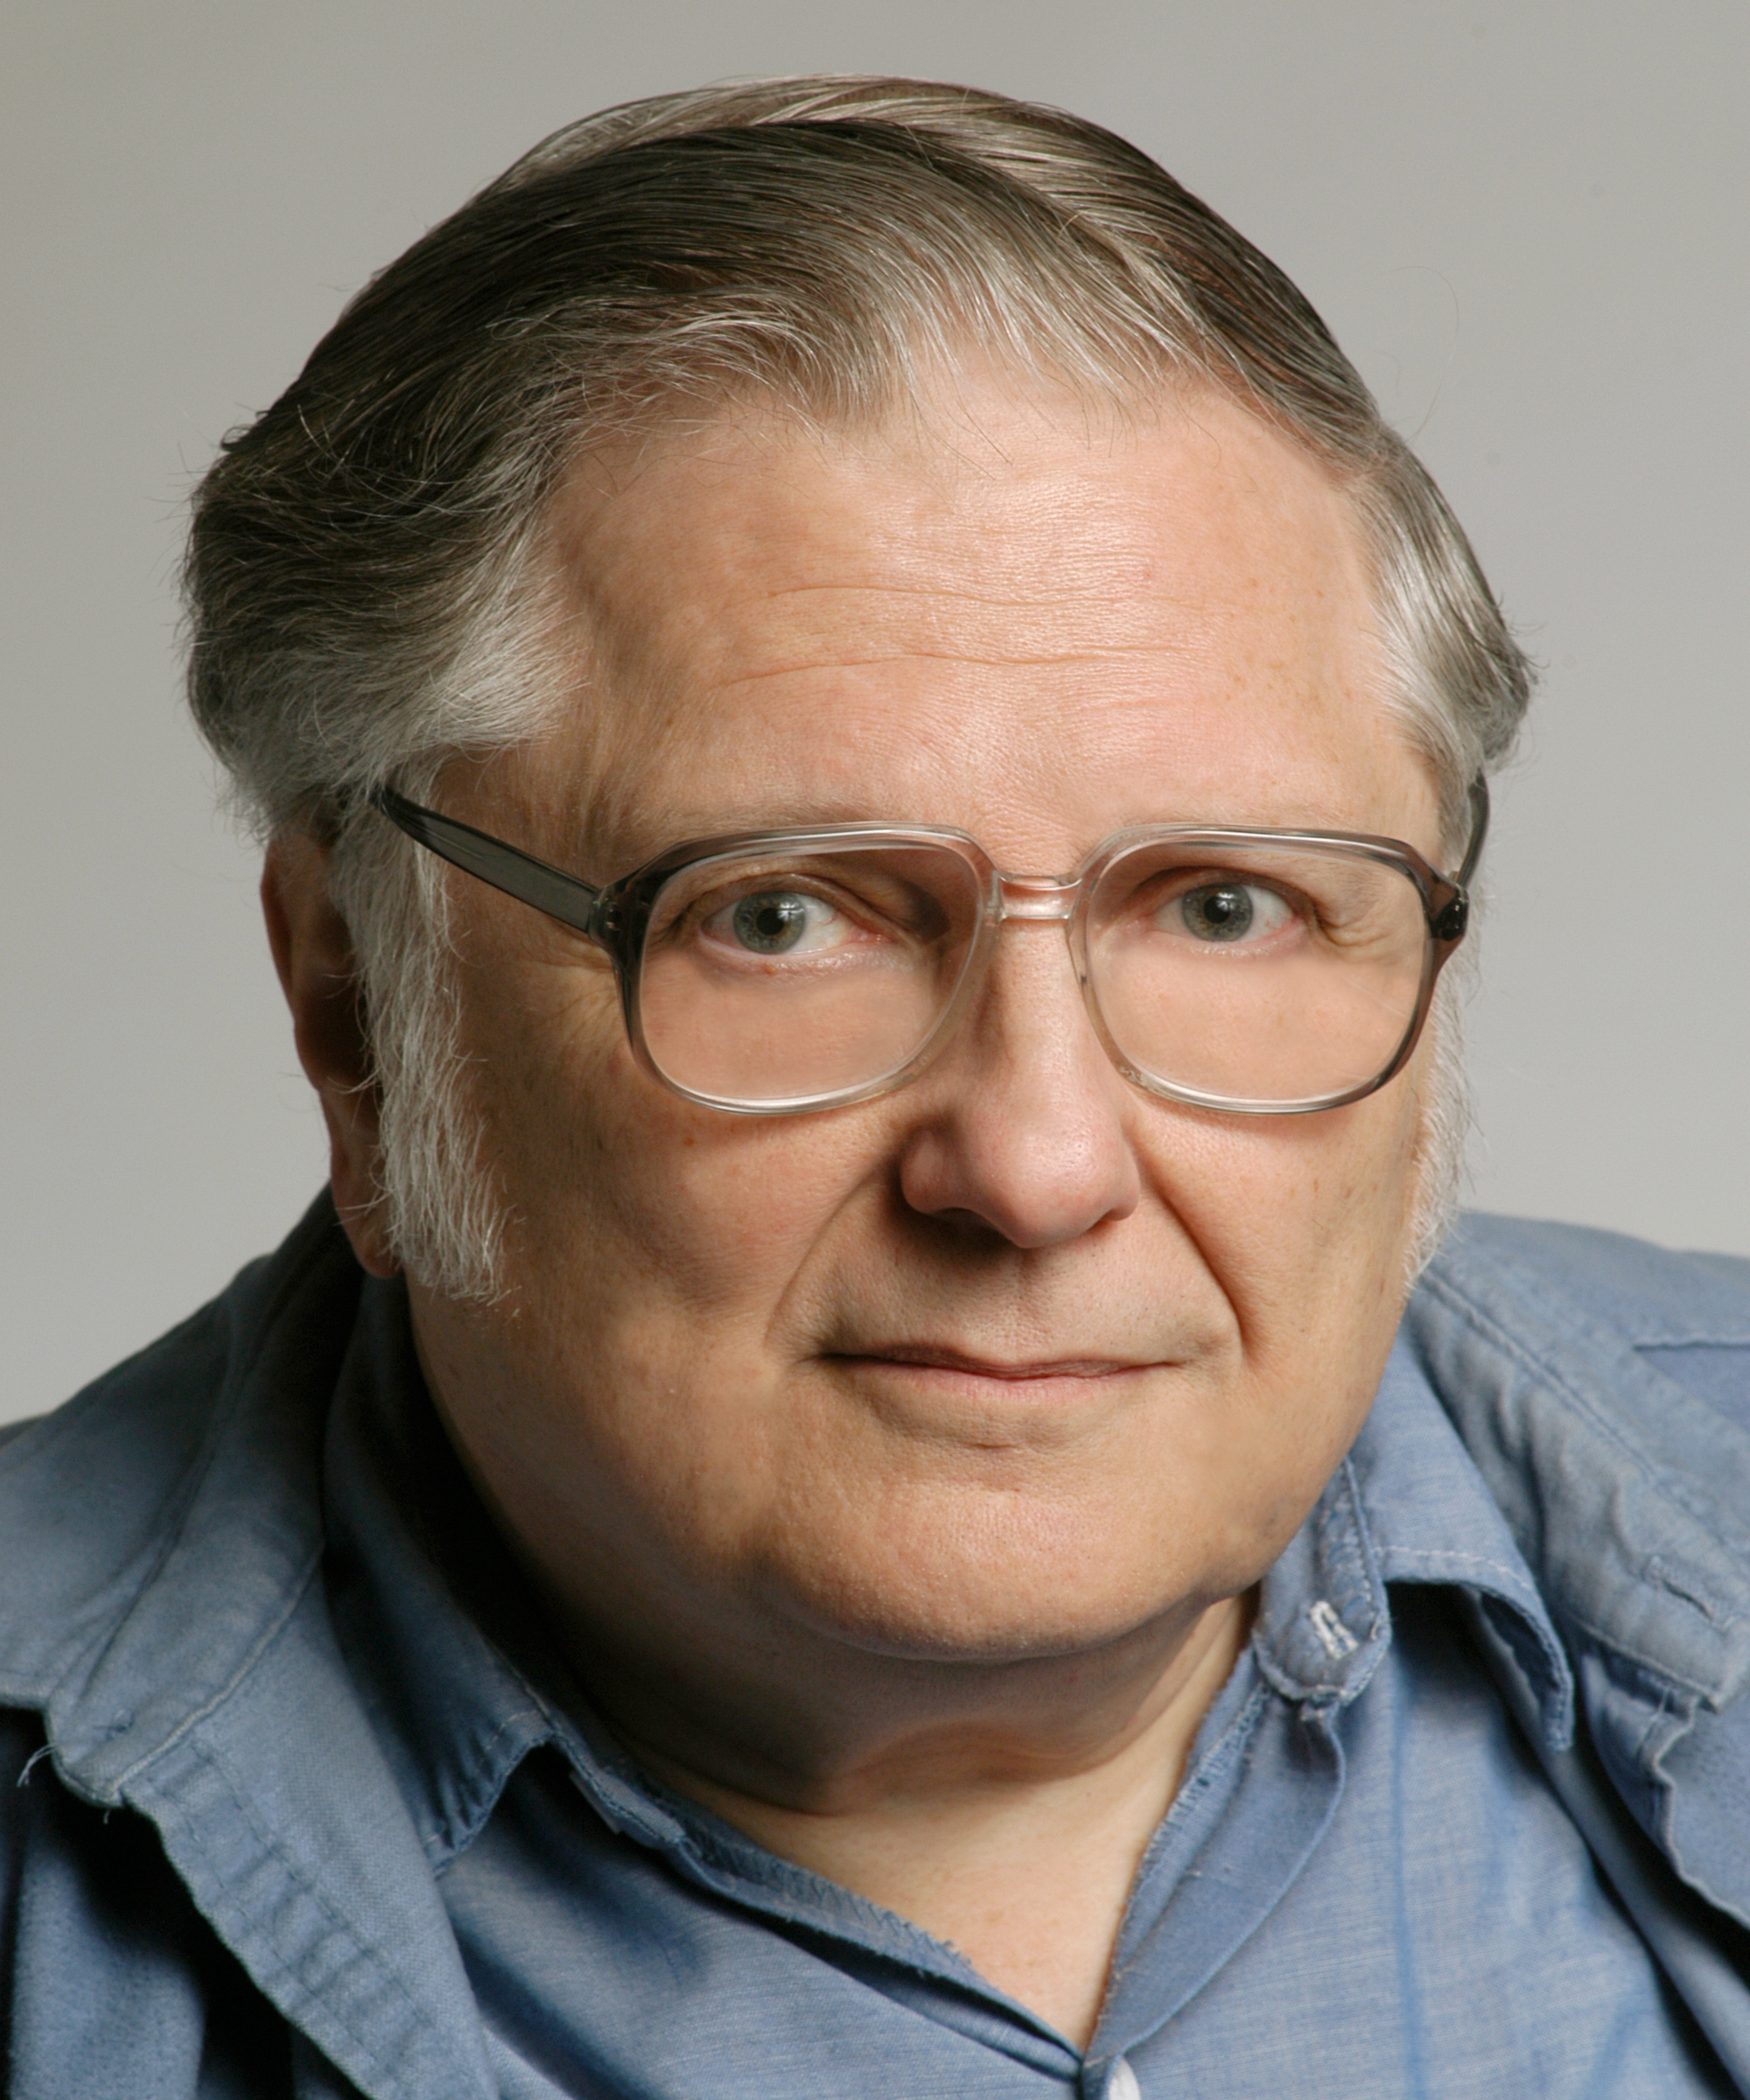
\includegraphics[width=0.7\linewidth]{pic_kahan}
					\label{fig:pickahan}
				\end{figure}
			\end{minipage}
			\hfill
		}
	\end{figure}
	
	\begin{figure}[H]
	\noindent\makebox[\textwidth][c]{%
		\begin{minipage}[H]{0.5\linewidth}
			\begin{figure}
				\centering
				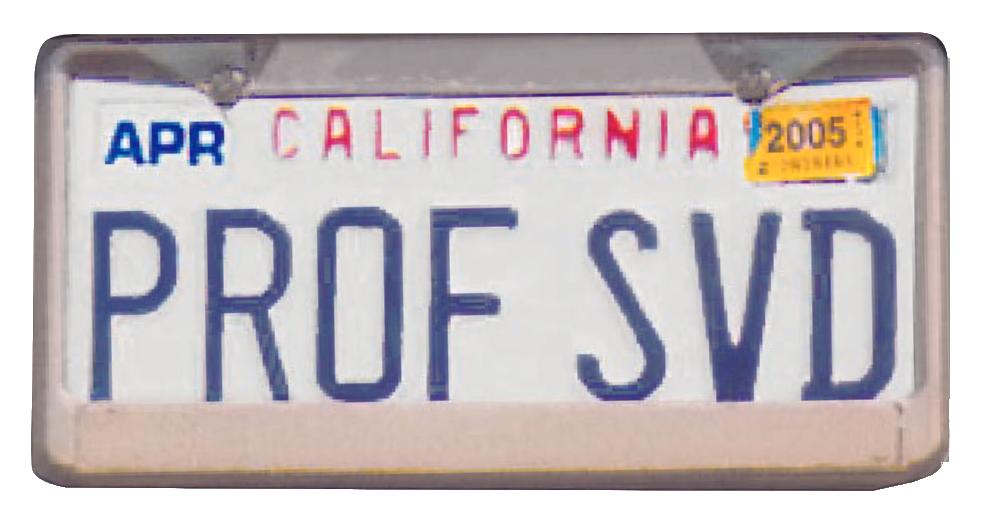
\includegraphics[width=0.5\linewidth]{pic_plate}
%				\caption{}
				\label{fig:picplate}
			\end{figure}
		\end{minipage}
		\begin{minipage}[H]{0.5\linewidth}

		\end{minipage}
		\hfill
	}
\end{figure}
	
	
	
	
	
	
\end{frame}



\begin{frame}{RX2}
	
	
	
	\begin{tikzpicture}[
	scale=1.4,
	MyPoints/.style={draw=blue,fill=white,thick},
	Segments/.style={draw=blue!50!red!70,thick},
	MyCircles/.style={green!50!blue!50,thin}, 
	every node/.style={scale=1}
	]
%	\draw[color=gray,step=1.0,dotted] (-8,-6) grid (8,6);
	\clip (-8,-6) rectangle (8,6);
	
	
	%\draw[->, >=stealth] (-1,0)--(6.5,0) node[right]{$x_1$};
	\draw[-{Latex[length=4.5mm, width=2.5mm]}, >=stealth] (0,-5)--(0,5) node[above left]{$x_2$};
	
	\draw[-{Latex[length=4.5mm, width=2.5mm]}, >=stealth] (-6,0)--(6,0) 
	node[right]{$x_1$};
	
	
	%{\verb!->!new, arrowhead = 2mm, line width=4pt}
	%, arrowhead = 3mm
	%, arrowhead = 0.2
	
	% Feel free to change here coordinates of points A and B
	\pgfmathparse{0}		\let\Xa\pgfmathresult
	\pgfmathparse{0}		\let\Ya\pgfmathresult
	\coordinate (A) at (\Xa,\Ya);
	
	\pgfmathparse{-1}		\let\Xb\pgfmathresult
	\pgfmathparse{1}		\let\Yb\pgfmathresult
	\coordinate (B) at (\Xb,\Yb);
	
	\pgfmathparse{1}		\let\Xc\pgfmathresult
	\pgfmathparse{1}		\let\Yc\pgfmathresult
	\coordinate (C) at (\Xc,\Yc);
	
	
	
	\draw[line width = 0.5mm, ->, vecb] (3, -3) -- (-3, 3) node[above right]{$p_{2}$};
	
	\draw[line width = 0.5mm, ->, vecb] (-4, -4) -- (4, 4) node[above left]{$p_{1}$};
	
	\tkzMarkRightAngle[size=0.3, vecb, line width = 0.3mm](B,A,C);
	
	
	\clip[rotate=45] (0, 0) ellipse (4 and 2);
	\foreach \p in {1,...,800}
	{ \fill[black, rotate = 45]  (0 + 4*rand,3*rand) circle (0.035);
	}
	
	
	
	
	
	
	\end{tikzpicture}
	
	
	
	
\end{frame}

\end{document}
